% IE 643 course project report, built on the course template (IE643_Project_Report.tex,
% Google Drive folder linked from the intensive-assessment instructions). The preamble and
% the \lecture header are the template's; only packages and macros were added.
%
% Build:  latexmk -pdf IE643_Project_Report.tex

\documentclass[twoside,english]{article}
\setlength{\oddsidemargin}{0.25 in}
\setlength{\evensidemargin}{-0.25 in}
\setlength{\topmargin}{-0.6 in}
\setlength{\textwidth}{6.5 in}
\setlength{\textheight}{8.5 in}
\setlength{\headsep}{0.75 in}
\setlength{\parindent}{0 in}
\setlength{\parskip}{0.1 in}

%
% ADD PACKAGES here:
%

\usepackage{amsmath,amsfonts,graphicx,algorithm,caption}
\usepackage[noend]{algpseudocode}
\usepackage{hyperref}
\usepackage{natbib}
\usepackage[document]{ragged2e}
\usepackage{graphicx} %package to manage images
\usepackage{amsmath}
\usepackage{mathtools}
\usepackage{xcolor}
\usepackage{booktabs}
\usepackage{tikz}
\usetikzlibrary{positioning,arrows.meta}
\setcitestyle{numbers,square}
\hypersetup{colorlinks=true,linkcolor=blue!50!black,citecolor=blue!50!black,urlcolor=blue!50!black}
\captionsetup{font=small}

% The following commands set up the lecnum (lecture number)
% counter and make various numbering schemes work relative
% to the lecture number.
%
\newcounter{lecnum}
\renewcommand{\thepage}{\arabic{page}}
\renewcommand{\thesection}{\arabic{section}}
\renewcommand{\theequation}{\arabic{equation}}
\renewcommand{\thefigure}{\arabic{figure}}
\renewcommand{\thetable}{\arabic{table}}
\makeatletter
\def\BState{\State\hskip-\ALG@thistlm}
\makeatother
%
% The following macro is used to generate the header.
%
\newcommand{\lecture}[4]{
   \pagestyle{myheadings}
   \thispagestyle{plain}
   \newpage
   %\setcounter{lecnum}{#1}
   \setcounter{page}{1}
   \noindent
   \begin{center}
   \framebox{
      \vbox{\vspace{2mm}
    \hbox to 6.28in { {\bf IE 643: Deep Learning - Theory and Practice
		\hfill July-Dec 2026} }
       \vspace{4mm}
       \hbox to 6.28in { {\Large \hfill Project Report: #1  \hfill} }
       \vspace{2mm}
       \vspace{2mm}
       \hbox to 6.28in { {\it Team Name: #2 \hfill Team Members: #3} }
      \vspace{2mm}}
   }
   \end{center}
   \vspace*{4mm}
}

\newtheorem{theorem}{Theorem}[lecnum]
\newenvironment{proof}{{\bf Proof:}}{\hfill\rule{2mm}{2mm}}

% **** IF YOU WANT TO DEFINE ADDITIONAL MACROS FOR YOURSELF, PUT THEM HERE:
\newcommand{\R}{\mathbb{R}}
\newcommand{\xs}{\bar{x}}         % frame mean (static part)
\newcommand{\xd}{\tilde{x}}       % frame-mean-removed residual (dynamic part)
\newcommand{\dD}{\Delta D}
\usepackage{url}
\DeclareUrlCommand\code{\urlstyle{tt}}
\newcommand{\todo}[1]{\textcolor{red}{[#1]}}

\begin{document}
\lecture{Probing Video Diffusion U-Nets for Content vs.\ Motion}{Claudn't}{\todo{roll numbers}}

\begin{abstract}
A text-to-video diffusion U-Net alternates spatial layers, which see one frame, with temporal
layers, which see all frames. We asked where inside such a model the content of a clip (what is
depicted) and its motion (how it moves) are actually decided, and whether that answer is good
enough to edit one without the other. We used AnimateDiff (Stable Diffusion 1.5 with a motion
adapter) and generated 360 clips in 750 controlled pairs in which a single prompt word changes
and the initial noise is fixed. From these pairs we built selectivity maps over 16 layers and all
25 denoising steps, and tested three hypotheses whose test statistics were fixed before the
data existed. Motion selectivity is weak almost everywhere; it peaks in the temporal module of
the first decoder block (\code{up_blocks.0}, 8$\times$8 latent) in 1000 of 1000 bootstrap
resamples, and only during the first 2--3 of 25 steps (changepoint $\tau=2$, 95\% CI [1,3]).
We then turned the static/dynamic split used for the maps into an intervention, a
\emph{component patch} that transplants only the frame-varying part $\xd$ or only the frame
mean $\xs$ of an activation between two generations. On 12 held-out test pairs the selected
component patches beat a prompt-only edit on the median in both directions
(median $\dD$ +0.041 and +0.068) and beat whole-tensor patching, but their 95\% confidence
intervals include zero, so our pre-registered success criterion is not met. Temporal-attention
injection, the training-free baseline, is the only method whose interval excludes zero: +0.105
(CI [0.001, 0.204]) over the first third of the steps, and +0.120 (CI [0.020, 0.203]) over all steps. We also trained motion LoRAs placed by the map and in a deliberately wrong
place. Across three seeds the map-guided LoRA is the only one with a positive median gain in every
seed, though the gain is small (+0.009 to +0.015) and not significant. We also built a Gradio
interface for live edits, uploaded videos and browsing every scored clip.
\end{abstract}

\section{Introduction}


Recent text-to-video diffusion models can easily turn a prompt into a short, realistic clip. Every such clip combines two things i.e. its \emph{content} which denotes
what is present in the frames, like a dog etc. , and its \emph{motion} which denotes how the content present in the frames is moving.  In principle the two are independent in the sense that
the same motion could be performed by a different object. For example instead of a dog running along a road you could have a horse running along the road. This project asks that at
whether a video diffusion model keeps them apart internally and if it does then in which layers and at which
denoising steps does it decide content and and ata which steps does it decide the motion, and whether that knowledge is precise enough to
change one while keeping the other.


Answering this question is important because people increasingly want to edit a generated clip rather than regenrating it because changing the prompt changes the subject, the background and motion all at once. 
Recent video diffusion models are built on image diffusion models by adding temporal layers to them, as AnimateDiff
\citep{guo2024animatediff} does with Stable Diffusion \citep{rombach2022ldm}. Recent editing
methods \citep{wu2023tav,zhao2024motiondirector,ling2025motionclone,xiao2024moft} intervene on
chosen layers or features to transfer or customise motion, but they chose those places by design or by ablation. The obvious reading by archtecture stating spatial and temporal layers 
is usually assumed rather than measured. A measured mapping of where the content lies and where the motion lies would allow targetted edits, changing only certain parts of the clip and retaining the other 
desired ones rather than entire regeneration of the clip. It would show us where to place the few trainable parameters of LoRA \citep{hu2022lora} when teaching the model a new motion. 
A negative answer is also useful because if the split is not clean then the editing methods that assume this clean split are working for some other reasons that need further invetsigation. 


To find such a map, we experiment with the model. The model is a U-net architecture that turns noise into video over a sequence of denoising steps. It was trained on just the input and the output and was never told 
as to which part of the model should carry the motion and which should carry the content. So any
such seperation should be something that it learned on its own and has to be located emperically because
it is spread across many high-dimensional layers and across many denoising steps so it cannot be read
by weights alone nor by the architecture diagram. 
Architectural diagrams labelling layers as spatial and temporal tells us what each layer \emph{can}
see not what it actually ends up encoding. 
Finding the seperation would require us to actually study the trained network by changing the input
in a controlled way and then observing how the activations are responding to those changes and then
testing whether the places we found really control the desired properties or by intervening on them
midst generation. We then use evalutations to judge whether the edits were successful or not.


The report is organised as follows. Section~\ref{sec:workflow} lists how the work progressed.
Section~\ref{sec:litsurvey} surveys the work we built on. Section~\ref{sec:our_proj} describes
the methods, split into work done before and after the prep-presentation review.
Section~\ref{sec:data} covers the data, Section~\ref{sec:exp} the experiments and their
settings, and Section~\ref{sec:results} the results. Section~\ref{sec:Plan for Novelty Assessment}
gives the plan for novelty assessment and Section~\ref{sec:conclusion} concludes.

\section{Project Workflow} \label{sec:workflow}

We started with the question of finding out where the content lives and where the motion lives.
The architecture suggests an easy answer that the appearance would be stored in the spatial layers and 
the motion would be stored in the temporal layers. But we wanted to test it out by measuring it. 
Our first experiments showed that the motion was harder to measure than we expected because pixels 
that move also change depending on the object performing the motion. We developed tools to look inside
the model when it generated clips and used those measurements to gauge where is content stored and
where is motion stored. And based on those observations we tried to edit the model mid generation to validate
our hypthesised places of residence of content/motion. Some of our predictions were correct
and some of them turned out to be false that told us what to try out next.

\begin{figure}[!h]
\centering
\begin{tikzpicture}[
  wf/.style={draw=black!60, rounded corners=2pt, align=center, font=\footnotesize,
             minimum height=1.25cm, text width=2.45cm, fill=#1},
  wf/.default=white, >={Stealth[length=2mm]}, node distance=0.55cm]
\node[wf=black!5] (q) {\textbf{Problem statement}\\where do content\\and motion live?};
\node[wf=black!5, right=of q] (pl) {\textbf{Planning}\\model,\\hypotheses,\\tests fixed early};
\node[wf=black!5, right=of pl] (pi) {\textbf{Pilot}\\\textbf{experiments}\\cost, motion\\confound, storage};
\node[wf=blue!8, right=of pi] (to) {\textbf{Probing tools}\\95 hooks,\\lockstep sampler};
\node[wf=blue!8, right=of to] (lo) {\textbf{Locating content}\\\textbf{and motion}\\360 clips, maps};
\node[wf=blue!8, below=1.1cm of q] (va) {\textbf{Other models}\\same probing on\\4 variants};
\node[wf=black!5, right=of va] (lr) {\textbf{Motion LoRAs}\\full / map-placed\\/ wrong place};
\node[wf=orange!12, right=of lr] (iv) {\textbf{Intervention}\\patches, attention\\injection, controls};
\node[wf=orange!12, right=of iv] (ed) {\textbf{Editing}\\4 dev pairs $\to$\\12 held-out pairs};
\node[wf=black!5, right=of ed] (in) {\textbf{Interface}\\live edit, upload,\\browser};
\draw[->] (q) -- (pl); \draw[->] (pl) -- (pi); \draw[->] (pi) -- (to); \draw[->] (to) -- (lo);
\coordinate (bus) at ([yshift=-0.55cm]lo.south);
\draw (lo.south) -- (bus);
\draw[->] (bus) -| (iv.north);
\draw[->] (bus) -| (lr.north);
\draw[->] (bus) -| (va.north);
\draw[->] (iv) -- (ed); \draw[->] (ed) -- (in);
\draw[->] (lr.south) -- ++(0,-0.35) -| (ed.south);
\path (pi.east) -- coordinate[midway] (rv) (to.west);
\draw[dashed, black!50] ([yshift=0.95cm]rv) -- ([yshift=-0.8cm]rv)
   node[pos=0, above, font=\scriptsize, black!70] {prep review (21 Sep)};
\end{tikzpicture}
\caption{Order of the work. Everything left of the dashed line was done before the
prep-presentation review. The maps from the probing decide where we intervene and where the
map-placed LoRA sits, and the same probing is then repeated on four other model variants.}
\label{fig:workflow_diagram}
\end{figure}

\begin{itemize}
\item \textbf{Problem framing:} Problem was to find out which layers store content and which of them
store motion of a video diffusion U-net model. Then use this information to edit a clip so that one 
of these is kept intact and the other is changed.
\item \textbf{Planning:} We defined what content meant and what motion meant so we could measure it 
properly, chose AnimateDiff as our model over ModelScope and Stable Video Diffusion because it has
  explicit spatial and temporal split and takes text prompts as input and we fixed our prompt, the variables we would change and three hypothesis that we would test before seeing any data. 
\item \textbf{Experiments:} 
 \begin{itemize}
  \item Measured the cost of generating each clip
  \item Found that the pixel space motion also depends on the object we are using to perform the motion
  which gave us the idea to measure motion on the residual of the frame mean for each frame
  \item Found out that storing the full activations required way too much  memory so we scored the pairs
  during generation itself.
  \end{itemize}
\item \textbf{Probing Tools:} Built a package that hooks into 95 modules of the U-net, wrote a sampler
that generated groups of clips thata were bit identical to the diffusers pipeline and built a runner 
for the Kaggle T4s.
\item \textbf{Locating content and motion:} Generated 360 clips that formed 750 pairs with the one word
swaped in the prompt. Then selectivity mas were created for each layer and steps. We tested Our
3 hypothesis and trained the linear probes. 
\item \textbf{Intervention Framework:} Built patches that transplant only the static or only the frame varying
part of the activation from one generation to another. Also built a temporal attention injection baseline.
\item \textbf{Editing:} Chose one configuration per direction on 4 pairs of development and scored it on 12 pairs. 
Added attention level edits and prompt switching. 
\item \textbf{Trained Model:} Trained motion LoRAs on where the map points and also where it does not.
After finding scene cuts in training clips we retrained.
\item \textbf{Check findings on other models:} We repeated the probing on 4 other model variants to
see if the map is specific to the diffusion model we used or does it apply in general.  
\item \textbf{Interface:} A live app where we can edit an uploaded video and view the maps and cross-attention
\end{itemize}

\section{Literature Survey} \label{sec:litsurvey}

Video is a stack of static frames that contain content. A video model hence would require two kinds of layers,
one that is spatial in nature that stores the content and one that is temporal in nature and stores the motion.

Video Diffusion Models \citep{ho2022vdm} built a video model this way. They 
extended the image U-Net architecture to a video generation architecture by factorising 
attention into a spatial part
and a temporal part. Video LDM \citep{blattmann2023align}
did the same in the latent space of Stable Diffusion \citep{rombach2022ldm} by keeping its weights fixed
and then inserted the temporal layers and trained only
the new layers. 

AnimateDiff \citep{guo2024animatediff} further built on this idea. People have their own fine tuned
image models each of which generated images in a particular style. AnimateDiff's goal was to make all of 
these image models produce 
its motion module
is a stack of temporal transformers trained once on video and then plugged into any
personalised Stable Diffusion 1.5 checkpoint without further tuning. This is why we chose it.
Content and motion sit in separate parameter sets by construction, so the structural
hypothesis ``spatial = content, temporal = motion'' is as clean as it can be in any open model,
and if it fails here it will not hold elsewhere. The catch is that the backbone never saw video
during training, so part of any separation we find may be a product of the recipe rather than
something a jointly trained model would learn. We return to this in
Section~\ref{sec:Plan for Novelty Assessment}.

\textbf{Activation patching.} Meng et al.\ \citep{meng2022rome} located factual associations in
GPT by running the model on a corrupted input and restoring one hidden state at a time from a
clean run (causal tracing); a state whose restoration recovers the answer is causally
implicated. Wang et al.\ \citep{wang2023ioi} used path patching to recover a full circuit
for a single task in GPT-2 small. Zhang and Nanda \citep{zhang2024patching} showed that the
conclusions depend on choices that are easy to make carelessly: how the input is corrupted,
which metric is used (probabilities versus logit differences), and whether one patches a
single layer or a window. We took three things from this line of work. We patch clean
activations from one generation into another rather than adding noise. We use windows of
denoising steps as well as single steps. And we run null and mis-indexed patches as controls
before trusting any effect.

\textbf{Motion inside video diffusion features.} Xiao et al.\ \citep{xiao2024moft} found that
removing the frame-mean component of a video diffusion U-Net's features, followed by a
channel selection, leaves a representation (MOFT) that encodes motion direction and can guide
generation without training. Their best features came from just after the first up-block.
This is the origin of our static/dynamic split and of hypothesis H1. MotionClone
\citep{ling2025motionclone} transfers motion from a reference video by guiding the temporal
attention maps of the generated video towards the reference's; Diffusion Motion Transfer
\citep{yatim2024dmt} does the same with a loss on space-time features. Both show that temporal
attention carries enough motion to transfer it. Our attention-injection baseline is
MotionClone's core idea in its simplest form: we replace the attention probabilities instead of
guiding towards them with gradients, which the brief's compute budget could not afford.

\textbf{Motion customisation by fine-tuning.} Tune-A-Video \citep{wu2023tav} and MotionDirector
\citep{zhao2024motiondirector} adapt a video model to a reference motion. MotionDirector uses a
dual-path LoRA \citep{hu2022lora}, one on the spatial layers for appearance and one on the
temporal layers for motion, so that the motion can be reused with new content. Our trained
model borrows the motion half and asks a narrower question: does a LoRA placed only where our
map says motion lives do as well as one placed everywhere?

\textbf{Attention as an explanation in image diffusion.} Prompt-to-Prompt \citep{hertz2023p2p}
edits images by reusing the cross-attention maps of one generation in another, and DAAM
\citep{tang2023daam} turns cross-attention into word-level heat maps. Both treat attention
maps as the place where layout is decided. Our timestep hypothesis H2 comes from the common
claim that diffusion models settle layout and motion early and appearance late, which
Baherwani et al.\ \citep{baherwani2025timesteps} tested for video diffusion, finding two regimes
over the denoising trajectory with a fairly consistent boundary between them.

\section{Proposed Approach} \label{sec:our_proj}

\subsection{Model and notation}

AnimateDiff consists of the frozen Stable Diffusion~1.5 U-Net (about 860\,M parameters) with
the motion adapter \code{guoyww/animatediff-motion-adapter-v1-5-2} \citep{hf_animatediff} (about 417\,M parameters) inserted after
the spatial layers of every block. The U-Net works on 4-channel latents of 64$\times$64
(for 512$\times$512 frames) and has four encoder blocks, a middle block and four decoder
blocks (Figure~\ref{fig:unet}). Each spatial transformer applies self-attention within a frame
and cross-attention to the CLIP text embedding. Each motion module reshapes the activation so
that the 16 frames become the sequence dimension, applies two temporal self-attention layers
with sinusoidal position encoding, and adds the result back to its input. There are 21 motion
modules (42 temporal attention layers) and 16 spatial transformer blocks. We call one hookable
output at one denoising step a \emph{coordinate}; the model has 95 hookable modules.

\begin{figure}[!h]
	\centering
	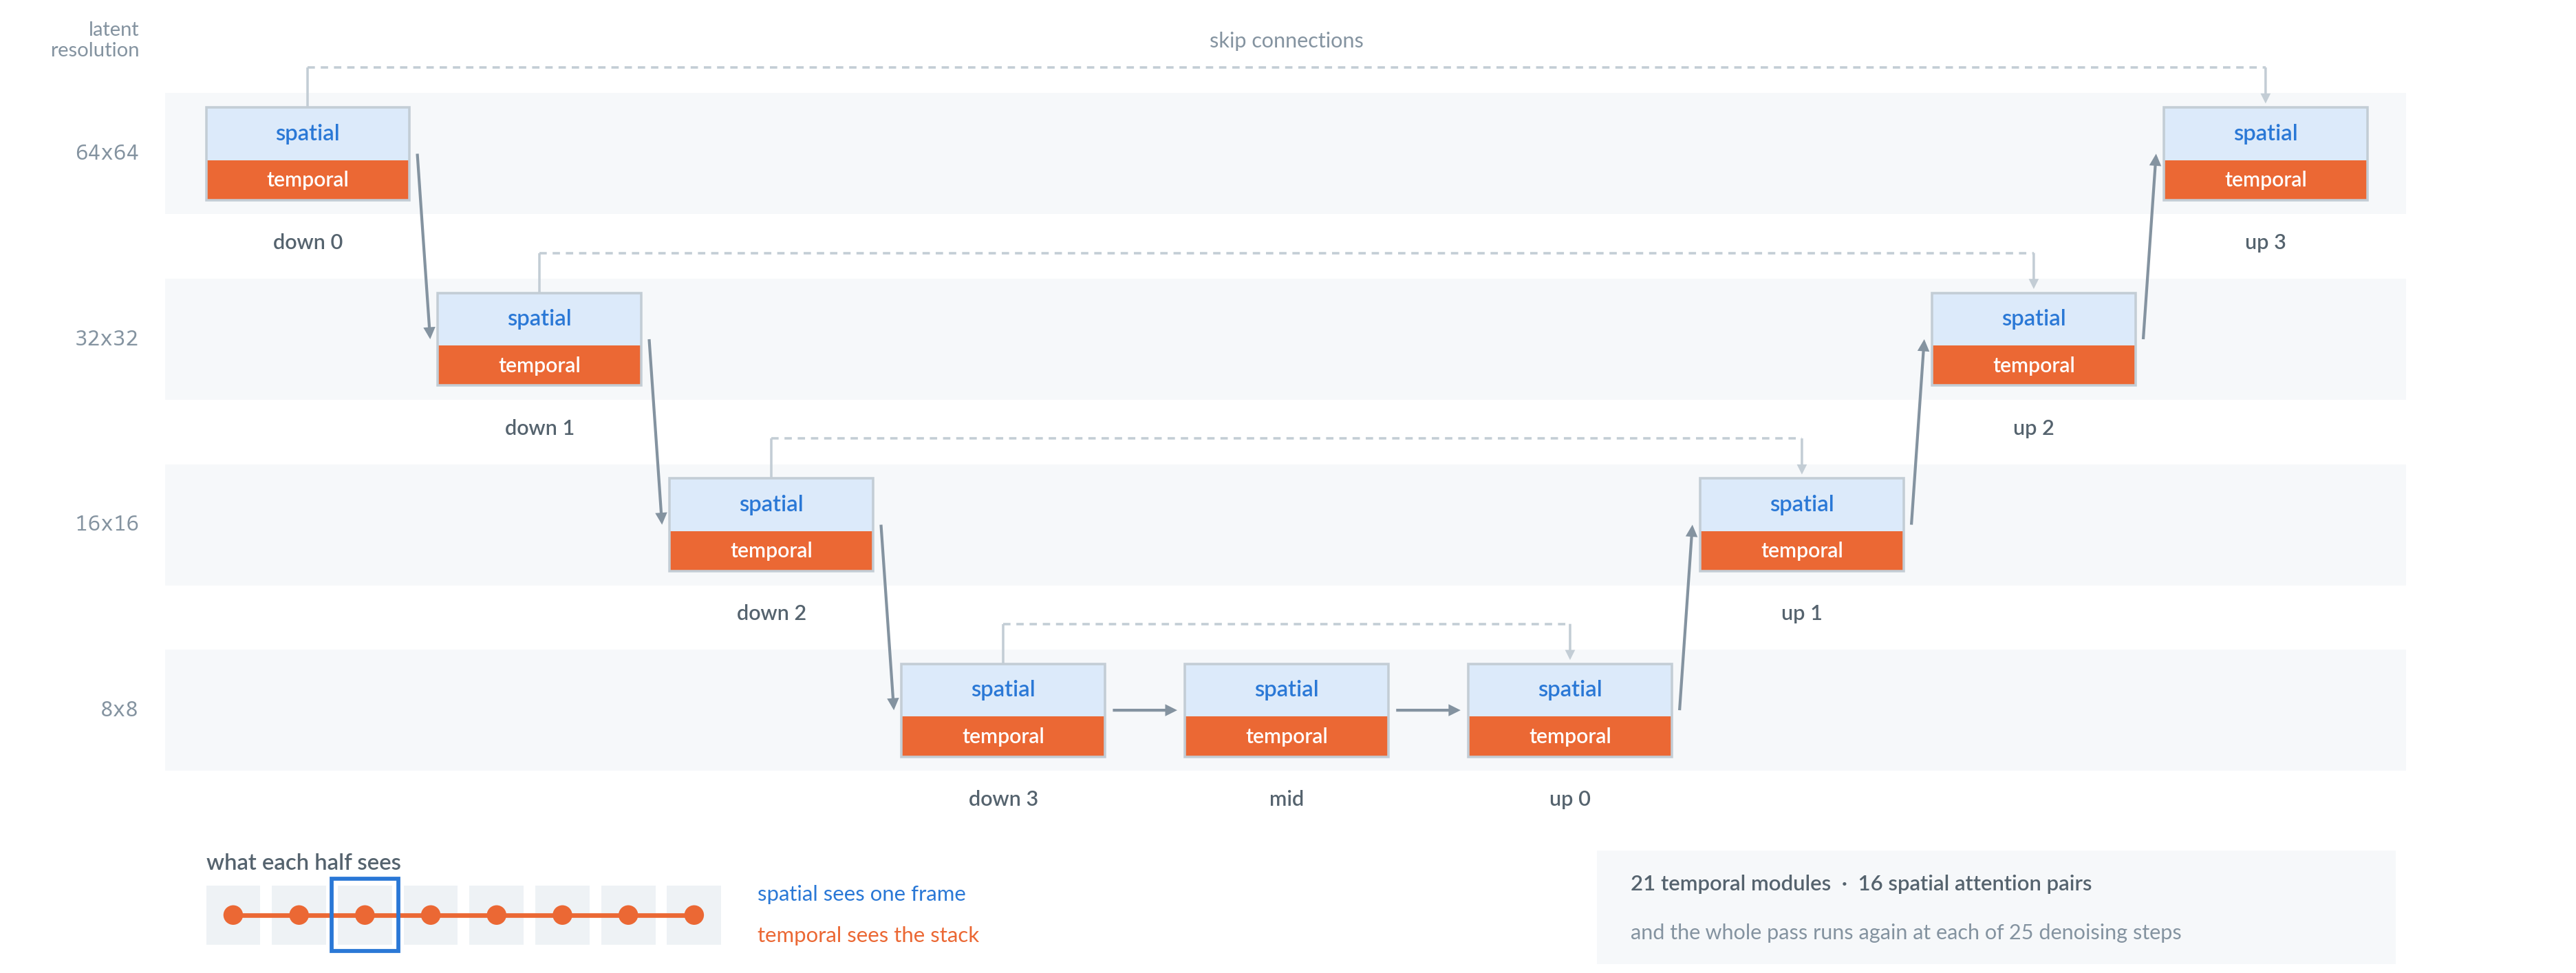
\includegraphics[width=\textwidth]{figures/unet.png}
	\caption{The AnimateDiff U-Net. Every block pairs spatial layers (one frame at a time) with
	a temporal motion module (all 16 frames at one position). The whole pass runs at each of the
	25 denoising steps. Block names in the text follow diffusers (\texttt{down\_blocks.0} \ldots
	\texttt{up\_blocks.3}); \texttt{up\_blocks.0} is the 8$\times$8 decoder block right after the bottleneck.}
	\label{fig:unet}
\end{figure}

Generation is fixed throughout (configuration frozen before the sweep): 16 frames, 512$\times$512,
25 DDIM steps \citep{song2021ddim}, classifier-free guidance scale 7.5, fp16, and the noise
tensor drawn on the CPU from a seed so that it is identical across machines.

For an activation at one coordinate we write it in a canonical form $x \in \R^{F\times C\times S}$
(frames, channels, spatial positions) and split it into
\begin{equation}
\xs = \frac{1}{F}\sum_{f=1}^{F} x_f, \qquad \xd = x - \xs, \label{eq:split}
\end{equation}
the static part, identical in every frame, and the frame-varying residual. For two clips $a,b$
generated from the same noise, with one prompt word different, the distance at a coordinate is
$d = 1-\cos(a,b)$ on the flattened tensor, computed separately on $\xs$ and on $\xd$.

\subsection{Work done before the prep-presentation review} \label{sec:before}

\textbf{Choice of model.} We compared three open models. AnimateDiff has an explicit
spatial/temporal split in its module tree, mature diffusers support, and fit on a T4 (10.2\,GB
measured). ModelScope T2V (1.7\,B parameters) trains space and time together end to end, which
makes it the harder and more interesting case, but the tooling for extracting its attention is
thinner. Stable Video Diffusion has the best output quality but is conditioned on an image only,
so we could not build matched pairs from one-word prompt changes. We chose AnimateDiff for all
deliverables and kept ModelScope as a later robustness check.

\textbf{Definitions and protocol.} From the brief we fixed: content is what an image
classifier would see in a single frame (subject identity, colour, texture, layout); motion is how
pixels move across frames, regardless of what they belong to. We wrote a roadmap with a register
of 22 decisions (D-01 to D-22), among them the distance (D-01: $1-\cos$), the static/dynamic
split (D-02), how pairs are formed (D-05), the edit metric and success criterion (D-14, D-16),
and the baseline (D-17).

\textbf{Three hypotheses with fixed tests.} Each one predicts something that could fail.
\begin{itemize}
\item \textbf{H1 (layer).} Motion selectivity peaks in a medium-resolution decoder block
  (\code{up_blocks.1}), following \citep{xiao2024moft}. Test: the bootstrap argmax over the
  nine temporal blocks of $M(b) = -\mathrm{mean}_t\,\mathrm{median}\,S_{dyn}(b,t)$ must
  exclude the extreme-resolution blocks.
\item \textbf{H2 (timestep).} Motion is settled early in denoising. Test: a single least-squares
  changepoint $\tau$ on the winning block's profile must fall in the first half, with the early
  segment above the late one.
\item \textbf{H3 (representation).} The frame mean $\xs$ is content-dominated, and removing it
  reveals motion selectivity that the raw activation hides. Test: at least 75\% of
  coordinate-steps have $S_{stat}$ significantly content-selective, and at least one temporal
  coordinate flips from content-selective in $\xs$ to motion-selective in $\xd$.
\end{itemize}

\textbf{Pilots E1--E3 (Kaggle T4).}
\begin{itemize}
\item \textbf{E1, cost.} 94.1\,s and 10.2\,GB per clip on a T4 at our settings, so the full
  360-clip probing set needs about 9.4 GPU-hours.
\item \textbf{E2, does a fixed noise tensor isolate a word?} Seven clips from one noise tensor:
  ``a golden retriever running on a beach'', three subject swaps and three verb swaps. Subject
  swaps moved CLIP appearance 2.6$\times$ more than verb swaps, so the content side of the
  control works. The motion side failed. A frame-difference motion proxy moved \emph{more} under
  subject swaps (0.461) than under verb swaps (0.390), because frame differences sit on the
  silhouette of the object and a new object has a new silhouette (Figure~\ref{fig:e2}). Pixel
  motion is confounded by content. This is why selectivity is measured on the frame-mean-removed
  residual, and why content pairs only swap subjects within a body-plan family (a dog for a wolf,
  not a dog for a person).
\item \textbf{E3, can we get the activations out?} Hooks on all 95 modules cost 0.6\% of
  generation time if they only record metadata. A full fp16 dump of every coordinate at every
  step is 87.9\,GiB per clip; a summary (channel statistics, per-frame residual norms, one
  16$\times$16 map per attention layer) is 44.6\,MiB, 2{,}017$\times$ smaller. Storing full
  activations for 360 clips was therefore impossible, which forced the online pair scoring
  described next.
\end{itemize}

\begin{figure}[!h]
	\centering
	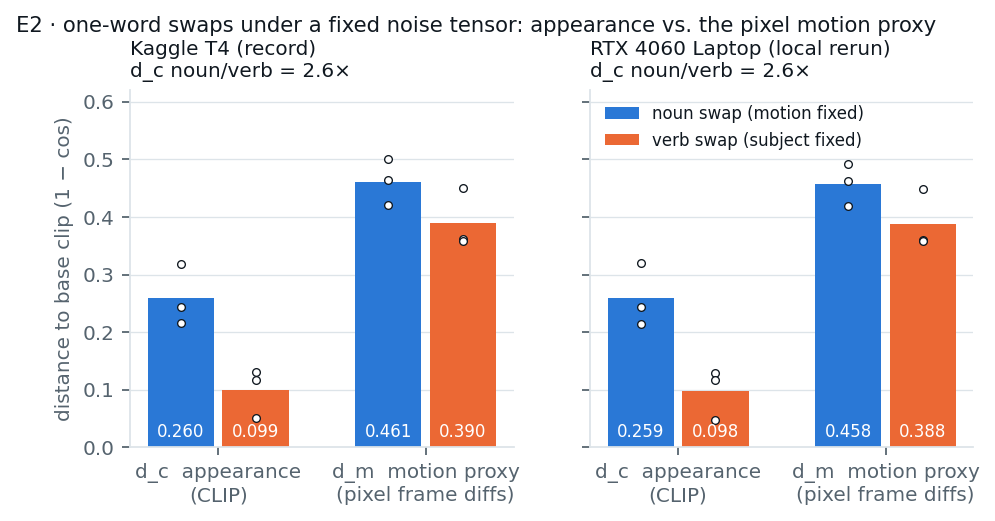
\includegraphics[width=0.82\textwidth]{figures/e2_pixel_confound.png}
	\caption{Pilot E2. A pixel-space motion proxy changes more when the subject is swapped
	(motion held fixed) than when the verb is swapped. Measuring motion in pixel space would have
	mistaken content for motion.}
	\label{fig:e2}
\end{figure}

\subsection{Work done after the prep-presentation review} \label{sec:after}

\textbf{Lockstep sampler and online scoring.} A selectivity map needs, for every pair, the
distance between two clips' activations at every coordinate and step. Caching the anchor clip's
activations at all 25 steps for 16 coordinates takes about 7.6\,GB of host memory per anchor,
and a group has 21 anchors. We instead denoise all 60 clips of a (seed, scene) group
\emph{in lockstep}: at step $t$ every anchor runs and its step-$t$ activations are kept, then
every partner runs and is scored against them, then the step-$t$ activations are dropped. Memory
holds one step instead of 25, every clip is generated exactly once, and the distances are
computed on the full tensors rather than on summaries. The loop re-implements diffusers'
\code{AnimateDiffPipeline} step by step (CFG concatenation, prompt-embedding repetition over
frames, the DDIM update). We verified it on the GPU before use: a clip generated alone, inside a
group, and with all probes attached gives a final latent identical to \code{pipe()} (mean
absolute difference exactly 0).

\textbf{Selectivity.} For one coordinate $(L,t)$, let $d_c$ be the distance across a content
pair (subject swapped) and $d_m$ across a motion pair (verb swapped). Then
\begin{equation}
S = \frac{d_c - d_m}{d_c + d_m} \in [-1, 1],
\end{equation}
positive when the coordinate tracks what is depicted and negative when it tracks how things move.
$S_{dyn}$ uses $\xd$ and $S_{stat}$ uses $\xs$. Since $d_c$ and $d_m$ come from different pairs,
we compute $S$ on matched units: a clip $B$ = (subject $s$, verb $v$, scene) that is the end point
of both a content pair (family anchor, $v$) $\to B$ and a motion pair ($s$, running) $\to B$. This
gives 78 units per seed. Each map cell is the median over units with a 1{,}000-sample bootstrap
CI within each seed, averaged over the three seeds.

\textbf{Linear probes.} To check whether motion information is \emph{present} even where
selectivity is low, we trained logistic-regression probes for the verb (4 classes) and the
subject's family (2 classes) on each coordinate and step. Storing full tensors was impossible, so
each clip's $\xd$ and $\xs$ were compressed with a count sketch to 512 dimensions, a random
projection that preserves inner products in expectation. Pipeline: standardise, PCA fitted on
the training split only, logistic regression ($C=1$). We trained on one scene and tested on the
other, so a probe cannot succeed by memorising the background.

\textbf{Component patching.} A patch replaces part of the target generation's activation at a
coordinate with the source generation's. Besides the usual whole-tensor, channel-subset and
$\alpha$-scaled patches, we added a \emph{component} patch that moves only one term of
Eq.~\eqref{eq:split}:
\begin{align}
\text{dynamic:}\quad & x_{out} \leftarrow \xs_{tgt} + \xd_{src}, &
\text{static:}\quad & x_{out} \leftarrow \xs_{src} + \xd_{tgt}.
\end{align}
The motion modules write into the residual stream, so a whole-tensor patch there copies content
and motion together. The split that defines the map is the natural way to move one and keep the
other. In fp16 the obvious implementation $\xs_{out} + x_{src} - \xs_{src}$ is not an exact
identity when source and target are the same clip; rounding errors grew over 25 steps to a
mean absolute difference of $10^{-2}$. We compute it instead as $x_{out} + (\delta - \bar\delta)$
with $\delta = x_{src} - x_{out}$, which is exactly zero for a self-patch.

\begin{algorithm}[!h]
\caption{One edit: source A and $N$ target arms denoised in lockstep from one noise tensor}
\label{alg:edit}
\begin{algorithmic}[1]
\Require noise $z_T$, prompts $p_A$ (source) and $p_{tgt}$, arms $\{(\text{coords}_k, \text{steps}_k, \text{component}_k, \alpha_k)\}_{k=1}^N$
\State $z^{A} \gets z_T$; \; $z^{k} \gets z_T$ for $k = 1..N$
\For{$t$ in the 25 DDIM steps}
  \State run U-Net on $z^{A}$ with $p_A$; cache A's outputs at every coordinate any arm patches at $t$
  \For{$k = 1..N$}
    \State run U-Net on $z^{k}$ with $p_{tgt}$; at each $c \in \text{coords}_k$, if $t \in \text{steps}_k$:
    \State \hspace{1em} $\delta \gets x^A_c - x^k_c$; \; $x^k_c \gets x^k_c + \alpha_k \cdot \mathrm{part}(\delta)$
      \Comment{part $=\delta-\bar\delta$ (dynamic), $\bar\delta$ (static) or $\delta$ (whole)}
    \State $z^{k} \gets \mathrm{DDIM}(z^{k}, \hat\epsilon^{k}, t)$
  \EndFor
  \State $z^{A} \gets \mathrm{DDIM}(z^{A}, \hat\epsilon^{A}, t)$; free the step-$t$ cache
\EndFor
\end{algorithmic}
\end{algorithm}

\textbf{Temporal attention injection (baseline).} In each temporal attention layer the target
uses the source's attention probabilities $P_{src}$ instead of its own over a chosen window of
steps, with its own values $V$. To keep a self-injection exactly null in fp16 we compute
$\mathrm{SDPA}(Q,K,V) + \alpha\, W_{out}\big((P_{src}-P)V\big)$, which equals
$\big((1-\alpha)P + \alpha P_{src}\big)V$ in exact arithmetic, with $P_{src}$ stored in fp32.

\textbf{Edit directions and the metric $D$.} Clips A and B differ in subject and verb. In the
\emph{motion} direction the target prompt is B's subject with A's verb and we patch $\xd$, so the
output should look like B and move like A. In the \emph{content} direction the target prompt is
A's subject with B's verb and we patch $\xs$. We score content fidelity $s_c$ as the mean
per-frame CLIP image cosine \citep{radford2021clip} and motion fidelity $s_m$ as the cosine of
dense Farneb\"ack optical-flow fields \citep{farneback2003} averaged over frame pairs. For the motion
direction
\begin{equation}
D = \tfrac12\big[\hat s_c(\text{out},B) + \hat s_m(\text{out},A)\big] - \tfrac12\big[\hat s_c(\text{out},A) + \hat s_m(\text{out},B)\big],
\end{equation}
with A and B exchanged for the content direction, and $\hat s$ min-max normalised over all values
in a run. $D$ rewards taking the right property from each clip and penalises taking the wrong one.
The quantity we report is $\dD = D(\text{arm}) - D(\text{prompt only})$ on the same pair: what the
patch adds over simply changing the prompt. The pre-registered success criterion (D-16) has three
parts: in both directions, the median $\dD$ is positive, its 95\% paired-bootstrap CI over pairs
excludes zero, and subject consistency stays within 10\% of the source clip's.

\textbf{Motion LoRAs (the trained model).} LoRA \citep{hu2022lora} adds a trainable low-rank update
$\Delta W = \frac{\alpha}{r}BA$ to frozen weight matrices. We put LoRA on the query, key, value and
output projections of the temporal attention layers, in three placements with the same rank,
data and number of steps:
\begin{itemize}
\item \code{full}: all 21 motion modules (9.67\,M trainable parameters);
\item \code{probe}: only \code{up_blocks.0}, the H1 bootstrap set (1.97\,M);
\item \code{anti}: \code{down_blocks.2} and \code{.3}, the two blocks with the lowest $M(b)$
  (2.62\,M, more than \code{probe}), a wrong-place control.
\end{itemize}
Without the control, ``\code{probe} is as good as \code{full}'' could mean that any block would do.
The loss is the standard $\epsilon$-prediction objective of the frozen model,
\begin{equation}
\mathcal{L} = \mathbb{E}_{z_0, \epsilon, t}\,\big\| \epsilon - \epsilon_\theta(\sqrt{\bar\alpha_t}\,z_0 + \sqrt{1-\bar\alpha_t}\,\epsilon,\ t,\ c) \big\|_2^2,
\end{equation}
on 16-frame VAE latents $z_0$ of real clips with caption $c$ = ``a person \{verb\}''; only the LoRA
matrices receive gradients.

\textbf{Interface.} The brief asks for an interface where a user can test the method on their
own inputs. We built a Gradio app (\code{scripts/app.py}) over an engine class
(\code{src/vdprobe/demo.py}) that loads AnimateDiff, CLIP and the LoRAs once on the first
request. It has four tabs.
\begin{itemize}
\item \textbf{Live edit.} The user picks clip A (subject, verb), clip B, a scene and a seed, a
  direction and a method: the selected component patch, a custom patch (any block, window and
  $\alpha$), whole-tensor patch, attention injection, or prompt + LoRA. The engine runs A, B,
  the prompt-only arm and the edit in one lockstep group, and shows the four clips with $s_c$,
  $s_m$ and $D$. A single edit has no pool of its own to normalise against, so $D$ uses the pool of
  the scored test run, and the app says so. Subjects and verbs are free text.
\item \textbf{Upload a video.} The user's video is cut to its longest shot (shot boundaries
  found from frame-difference jumps), resampled to 16 frames, encoded, and DDIM-inverted onto the
  sampler's 25 timesteps. The inverted trajectory then serves as the motion source for a new
  subject given in a prompt. The default method and starting noise for this path were chosen by
  experiment (Section~\ref{sec:res_upload}).
\item \textbf{Results browser.} Every clip of the dev and test sweeps with its scores and the run summary.
\item \textbf{Where motion lives.} The $S_{dyn}$ and $S_{stat}$ curves for each coordinate and
  the H1--H3 verdicts.
\end{itemize}
Every live edit is saved with its GIFs, scores and the full request, so a result shown in the
app can be reproduced.

\section{Data set Details} \label{sec:data}

\textbf{Generated probing set (main data).} The probing data are videos generated by the model
itself, from the prompt template ``a \{subject\} \{verb\} \{scene\}, high quality, detailed''.
Vocabulary, frozen on 22 Sep: 15 subjects in two body-plan families (quadrupeds: golden retriever,
German shepherd, horse, wolf, tiger, fox, deer, brown bear; humans: young man, young woman,
athlete, soldier, dancer, child, elderly man), 4 verbs (running, walking, jumping, spinning),
2 scenes (on a beach, in a forest), 3 seeds (42, 1337, 2024). That is 120 clips per seed and
360 in total, each 16 frames of 512$\times$512 RGB. Within a (seed, scene) group every clip
shares the same initial noise tensor, so two clips that differ in one word differ only because
of that word. Pairs per seed: 104 content pairs (subject swapped within a family, verb fixed),
90 motion pairs (verb swapped, subject fixed) and 56 cross-family pairs, reported separately as
a harder subset. Across the three seeds this gives 750 pairs and 300{,}000 distance rows (16
coordinates $\times$ 25 steps per pair). There is no download and no preprocessing beyond the
model's own VAE decoding; the data are regenerated exactly from the configuration files.

\textbf{Edit pairs.} 12 test pairs and 4 separate dev pairs (\code{configs/edit_pairs.yaml}),
frozen before any edit ran. In each pair A and B differ in both subject and verb; the test pairs
have 6 per family, use every verb on both sides, and cycle through scenes and seeds. The dev
pairs are used only to choose the patch configuration, so the test pairs never influence it.

\textbf{HMDB51 clips for the LoRAs.} Real human-action videos from HMDB51 \citep{kuehne2011hmdb},
fetched from the Hugging Face mirror \code{divm/hmdb51} \citep{hf_hmdb} at a pinned revision.
HMDB51 has about 6{,}800 clips in 51 action classes, collected from films and web video; the
clips we use are 240 pixels high at 30\,fps. We
use four classes that match our verbs (run, walk, jump, turn $\to$ spinning) and filter on
HMDB's own metadata tags: full body visible, no camera motion, one person, quality not bad, at
most one clip per source film. That leaves 19 clips (run 5, walk 5, jump 4, turn 5), 21 to 168
frames each, 2.0\,MB in total, recorded with SHA-256 hashes in \code{data/hmdb51_lora/manifest.json}.
The last clip of each class (sorted by name) is held out for validation: 15 train, 4 validation.

Preprocessing: 16 frames at stride $\min(2, \lfloor (n-1)/15 \rfloor)$ from a random start, a random
square crop of full height, resizing to 256$\times$256 with antialiasing, scaling to $[-1,1]$, and
encoding with the frozen VAE. Validation uses a fixed window and a centre crop. While debugging the
upload path we found that 11 of the 19 clips contain a hard scene cut (a mean grey-level jump
larger than both 4$\times$ the clip's median and 20). In the first recipe some training windows
spanned a cut. The \emph{cut-free} recipe (D-34) draws every window inside a single shot of at
least 16 frames, chosen with probability proportional to its length; a clip without such a shot
uses its longest shot with the last frame repeated.

\section{Experiments} \label{sec:exp}

\textbf{Hardware and software.} A laptop RTX 4060 (8\,GB, 15\,GB RAM) for development, controls,
LoRA training (first recipe), scoring and the interface; Kaggle sessions with 2$\times$ Tesla
T4 (16\,GB each) for the sweeps and the cut-free LoRAs, one job per GPU. Python 3.10, PyTorch
2.10 (2.11 on Kaggle), diffusers 0.40.0 \citep{hf_diffusers}, transformers 5.20, PEFT 0.21.2, scikit-learn 1.7.2,
OpenCV, Gradio 6.30. Every result file records the software versions, GPU, timings, peak memory,
and the resolved model repository and commit hash. One clip costs 65\,s on the laptop and
90--97\,s on a T4.

\textbf{Code.} \url{https://github.com/rujulaaaa/IE643}. The README lists the command for every
stage. The suite of 51 CPU tests runs on a tiny random U-Net in about 10\,s and covers hooks,
patches, controls, the analysis on a synthetic sweep with a planted answer, the metrics and the
interface engine.

\textbf{E4. Lockstep verification.} Four checks against \code{pipe()}: two \code{pipe()} runs
(floor), a solo lockstep clip, a clip inside a three-clip group, and a clip with all probes
attached. All four final latents matched exactly. A self-pair gave distances below
$3\times10^{-7}$; a verb swap gave a median $d$ of 0.555 on $\xd$ and 0.083 on $\xs$.

\textbf{E5. Probing sweep.} Six lockstep groups of 60 clips (3 seeds $\times$ 2 scenes), 16 coarse
coordinates $\times$ 25 steps. The coordinates are one representative per block: the last motion
module of each of the 9 blocks, and the cross-attention of the last spatial transformer of each of
the 7 blocks that have one (the last module is closest to the block output, and cross-attention
is where the prompt enters the spatial path). Kaggle, 2$\times$T4, 5.2 hours. Analysis on the CPU:
1{,}000 bootstrap resamples, probes in 836\,s.

\textbf{E6. Patching controls on the real model.} Null patches (source = target) for every patch
type; a mis-indexed null patch (the source's activation from two steps earlier), which
\emph{must} fail; an unpatched arm compared with the same clip generated as another group's
source; and a symmetry check, A$\to$B against B$\to$A on \code{up_blocks.0} over the first third
of the steps. The first run of these controls failed two of them. The component null patch
gave a mean absolute difference of $10^{-2}$ (the fp16 identity issue above). Attention recording
perturbed the source clip by $6\times10^{-3}$, because the recorder returned its own
explicit-softmax output instead of the stock one. A second run left the null attention
injection at $2.3\times10^{-3}$, which led to the $\mathrm{SDPA} + \alpha W_{out}(\cdot)$ form. The
third run is the run of record (Table~\ref{tab:controls}).

\textbf{E7. Dev sweep (configuration selection).} 4 dev pairs, 51 arms each: component patches on
the motion-module outputs of each of the 9 temporal blocks over two windows (first third of the
steps, i.e.\ steps 0--8; all 25), on all 21 motion modules over four windows (one step, five steps,
first third, all), both directions, plus whole-tensor and attention-injection references. Rule
(D-31, fixed before scoring): per direction, the component arm with the largest median $\dD$
among those whose median subject-consistency ratio is $\ge 0.9$, ties going to fewer modules.
Kaggle, 2.6\,h. Selected: motion, $\xd$ patch on \code{up_blocks.3} motion modules, steps 0--8
(dev median $\dD$ +0.080); content, $\xs$ patch on \code{down_blocks.3} motion modules, steps
0--8 (+0.015).

\textbf{E8. Test sweep.} 12 test pairs, 18 clips each: source, B, and per direction the prompt-only
arm, the selected patch, the selected patch at $\alpha \in \{0.25, 0.5, 0.75\}$, the whole-tensor
patch at the same place; temporal attention injection over steps 0--8 in all 42 temporal attention
layers; prompt + each of the three LoRAs. Kaggle, 10{,}017\,s. The first submission failed before
generating anything because the Kaggle image's \code{torchao} was incompatible with the newest PEFT;
we pinned PEFT 0.21.2 and removed \code{torchao}. Scoring (VAE decode, CLIP, optical flow) ran on the
laptop in 15 minutes, with 10{,}000 paired bootstrap resamples per CI.

\textbf{E9. Motion LoRAs, first recipe.} Rank 32, $\alpha=32$, Gaussian initialisation, AdamW
(learning rate $5\times10^{-5}$, weight decay $10^{-2}$), batch 1, 800 steps, timesteps uniform over
the 1{,}000 training steps, fp16 frozen weights with fp32 LoRA weights under autocast, seed 0. The
first attempt ran out of memory on the 8\,GB GPU at step 1: diffusers' gradient checkpointing
covers only the ResNets of this model, not the motion modules where the LoRA sits. We wrapped every
motion module in non-reentrant checkpointing (same gradients); peak memory fell to 5.0\,GB. 17--22
minutes per variant. Validation: the 4 held-out clips at 8 fixed timesteps $\times$ 2 fixed noise
tensors, identical for every variant and for the untrained model.

\textbf{E10. Motion LoRAs, cut-free with three seeds (D-34).} The same recipe with cut-free
windows, seeds 0, 1 and 2, nine LoRAs, on Kaggle (22--30 minutes each on a T4). On the 12 test
pairs we generated one prompt + LoRA arm per LoRA and attention injection over all 25 steps (the
best motion arm in the dev sweep, which the selection rule did not allow us to pick), regenerated
the source, B and the prompt-only arm, and scored everything in one pool with E8.
Kaggle, 2$\times$T4: about 1.9\,h of training and then 1.7--2.0\,h of edits per GPU.

\textbf{E11. Upload path.} Interface checks on real HMDB51 clips, comparing three starting points
for the new clip (the inverted noise, a unit-variance blend of the inverted and a Gaussian noise,
Gaussian noise alone) and three methods (selected $\xd$ patch, attention injection over the first
third, attention injection over all steps).

\section{Results}\label{sec:results}

\subsection{Where content and motion live}

\begin{figure}[!h]
	\centering
	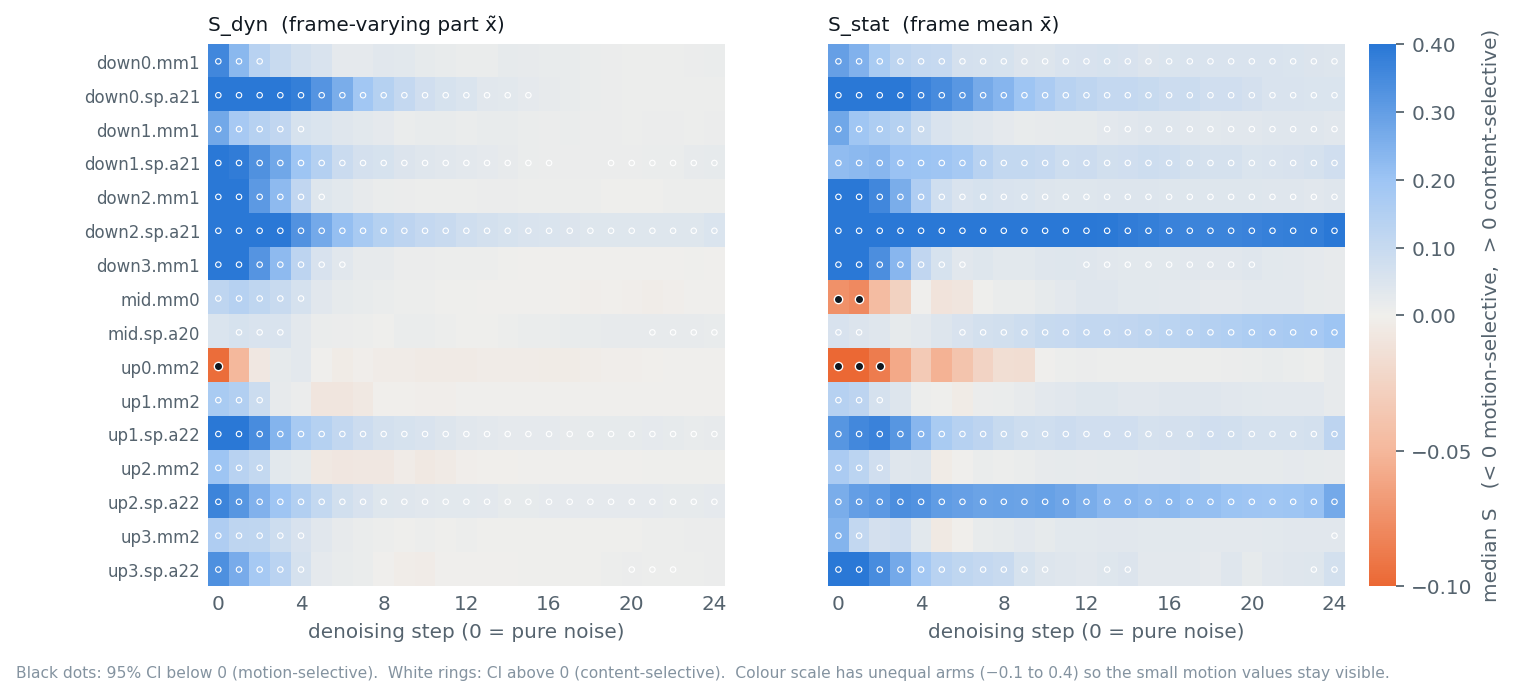
\includegraphics[width=\textwidth]{figures/sweep_selectivity_maps.png}
	\caption{Selectivity maps over 16 coordinates and 25 denoising steps (\texttt{mm} = motion module,
	\texttt{sp.a2x} = spatial cross-attention). Left: $S_{dyn}$ on the frame-varying part. Right:
	$S_{stat}$ on the frame mean. Blue is content-selective, orange motion-selective. Only
	\texttt{up0.mm2} (and \texttt{mid.mm0} in $\xs$) is motion-selective, and only in the first steps.}
	\label{fig:maps}
\end{figure}

Figure~\ref{fig:maps} is the central result of the probing stage. Almost every cell is blue: a
subject swap moves almost every layer more than a verb swap does, including the temporal layers.
The spatial cross-attention layers are the most content-selective. Every map fades towards zero
after about step 9, where content and motion swaps move the activations by similar amounts.
Table~\ref{tab:hyp} gives the three pre-registered tests.

\begin{table}[!h]
\centering
\small
\begin{tabular}{p{3.1cm}p{1.6cm}p{10.2cm}}
\toprule
Hypothesis & Verdict & Evidence \\
\midrule
H1: motion peaks at \code{up_blocks.1} & falsified & $M(b)$ is highest at \code{up_blocks.0} (+0.005), the argmax in 1000/1000 resamples. Every other block is negative: \code{up1} $-$0.017, \code{up2} $-$0.019, \code{mid} $-$0.026, \code{down0} $-$0.052, \code{down2} $-$0.075. The peak is sharp but at the extreme (8$\times$8) resolution the test excluded. \\
H2: motion is settled early & survives & On \code{up0.mm2}, $m(t)$ = 0.096, 0.050, 0.007, then about 0. Changepoint $\tau = 2$, 95\% CI [1, 3]; early mean 0.073 vs.\ late $-$0.001. \\
H3: removing $\xs$ reveals hidden motion & falsified & $f_{stat} = 0.65 < 0.75$ and no coordinate flips. $S_{dyn} < S_{stat}$ almost everywhere (e.g.\ \code{down2} cross-attention 0.43 $\to$ 0.17), so the split moves every coordinate towards motion, but never past zero. \\
\bottomrule
\end{tabular}
\caption{Pre-registered hypothesis tests (78 matched units per seed, 3 seeds, 1{,}000 bootstrap resamples).}
\label{tab:hyp}
\end{table}

\begin{figure}[!h]
	\centering
	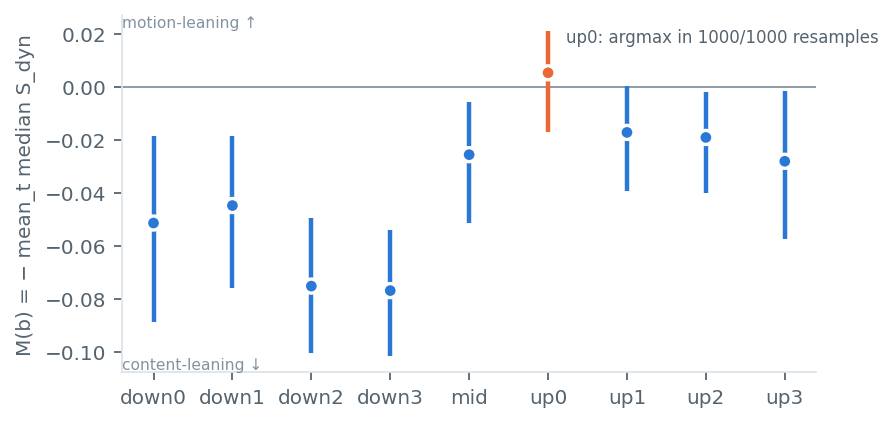
\includegraphics[width=0.49\textwidth]{figures/sweep_h1_blocks.png}\hfill
	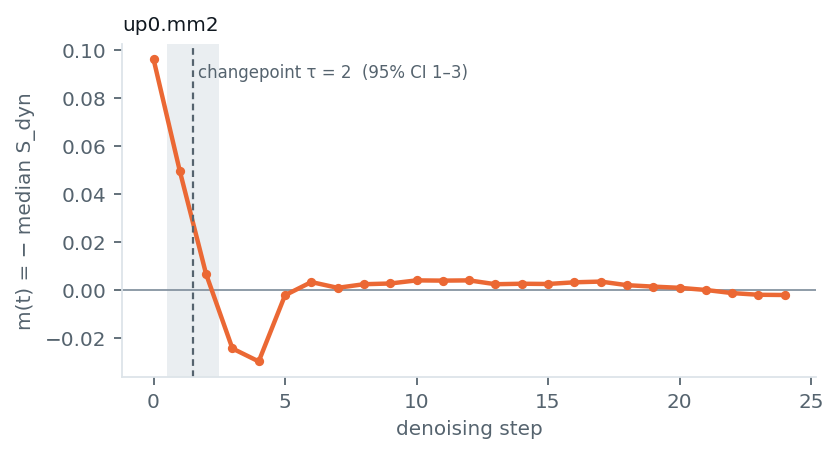
\includegraphics[width=0.49\textwidth]{figures/sweep_h2_timestep.png}
	\caption{Left: motion selectivity $M(b)$ of the nine temporal blocks with 95\% CIs; only
	\texttt{up\_blocks.0} is above zero. Right: the motion-selectivity profile of \texttt{up0.mm2} over
	the denoising steps, with the fitted changepoint and its CI.}
	\label{fig:h1h2}
\end{figure}

Two observations go beyond the tests. First, the H3 result is the opposite of what we expected:
at the very first steps the cleaner motion signal is in $\xs$, not $\xd$. $S_{stat}$ has five
motion-significant cells (\code{up0.mm2} at steps 0--2, \code{mid.mm0} at steps 0--1) and
$S_{dyn}$ only one. The static share of the activation energy, $F\|\xs\|^2/\|x\|^2$, is 0.39--0.70
in the motion modules but 0.82--0.9996 in the spatial cross-attention layers, so ``the frame mean is
content'' holds on the spatial path, not the temporal one. Second, on \code{up0.mm2} the motion
profile dips below zero at steps 3--4 ($-$0.024, $-$0.030) before settling. Our two-segment test was
not designed to detect that, and we have not interpreted it.

\textbf{Robustness.} Cosine and relative-L2 distances give nearly the same map (Spearman 0.987),
and the median of per-unit ratios agrees with the ratio of medians (0.930). Seed-to-seed agreement of
the $S_{dyn}$ map is only moderate (0.58, 0.69, 0.73), so cell-level detail should not be over-read.

\textbf{Linear probes.} With the scene split, the verb is decodable well above chance (0.25) in
places, for example 0.74 on the mid-block cross-attention (Figure~\ref{fig:probes}). Much of this is
the verb token leaking through the prompt: on that coordinate the probe on $\xs$ stays at 1.0 at every
step, because cross-attention reads the text embedding directly. On the temporal modules the frame
mean also decodes the verb better than the residual at every step. Selectivity and decodability are
different questions: a layer can carry the verb and still respond more to a change of subject.

\begin{figure}[!h]
	\centering
	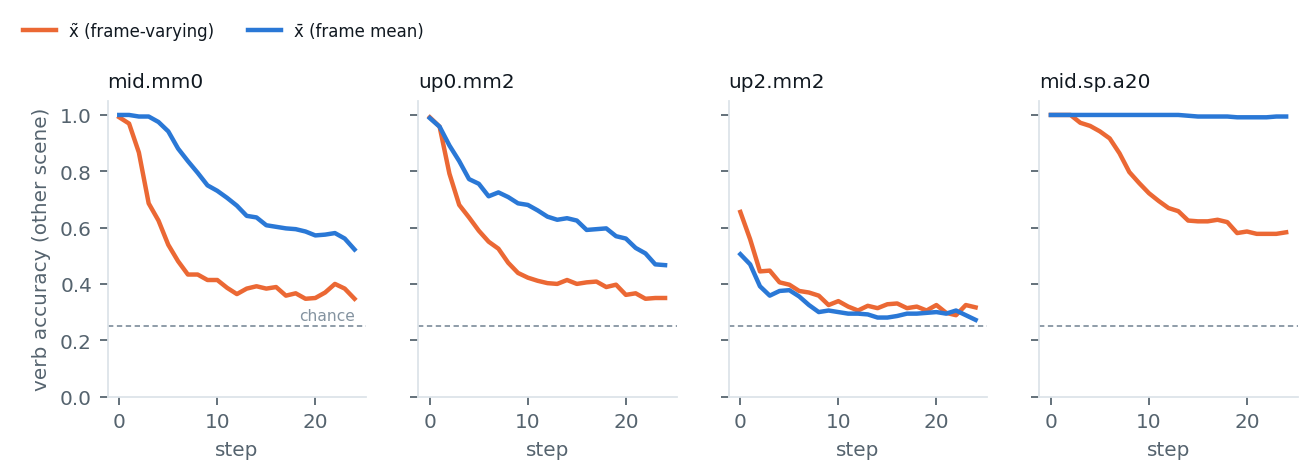
\includegraphics[width=0.8\textwidth]{figures/sweep_probes.png}
	\caption{Verb-probe accuracy over the denoising steps on four coordinates, trained on one scene and
	tested on the other (chance 0.25). $\xs$ decodes the verb at least as well as $\xd$ everywhere.}
	\label{fig:probes}
\end{figure}

\subsection{Patching controls}

\begin{table}[!h]
\centering
\small
\begin{tabular}{lll}
\toprule
Control & Result & Verdict \\
\midrule
Null patch: whole tensor, $\xd$ only, $\xs$ only, attention injection & MAD 0, PSNR $\infty$ & pass \\
Mis-indexed null patch (source from 2 steps earlier) & MAD 0.103, PSNR 25.1\,dB & detected, as required \\
Unpatched arm vs.\ the same clip as another group's source & MAD 0 & pass (no leakage) \\
Symmetry, \code{up_blocks.0}, steps 0--8: $f(A\to B)$ vs.\ $f(B\to A)$ & 0.171 vs.\ 0.083 & fail (ratio 2.06 $>$ 2) \\
\bottomrule
\end{tabular}
\caption{Controls on the real model (run of record). MAD = mean absolute difference of the final latents.}
\label{tab:controls}
\end{table}

The patching machinery is exact: every null patch reproduces the unpatched clip bit for bit, and
a deliberately wrong patch is caught. The symmetry control fails our own criterion. The effect has the
same sign both ways, but moving the golden retriever's run into the walking horse transfers twice as
much as the reverse. One explanation is that a running clip has more motion to move; we tested only one
pair, so this stays a conjecture.

\subsection{Edits on the held-out test pairs}

\begin{table}[!h]
\centering
\small
\begin{tabular}{llcccc}
\toprule
Direction & Arm & median $D$ & median $\dD$ & $\dD>0$ & 95\% CI \\
\midrule
keep A's motion & prompt only & 0.149 & 0 & -- & -- \\
 & $\xd$ patch, \code{up_blocks.3}, steps 0--8 (selected) & 0.195 & +0.041 & 8/12 & [$-$0.027, 0.143] \\
 & $\xd$ patch at $\alpha$ = 0.5 & 0.236 & +0.038 & 9/12 & includes 0 \\
 & whole-tensor patch, same place & 0.074 & $-$0.036 & 5/12 & [$-$0.109, 0.047] \\
 & attention injection, steps 0--8 (baseline) & 0.269 & \textbf{+0.105} & 10/12 & \textbf{[0.001, 0.204]} \\
\midrule
keep A's content & prompt only & 0.090 & 0 & -- & -- \\
 & $\xs$ patch, \code{down_blocks.3}, steps 0--8 (selected) & 0.198 & +0.068 & 10/12 & [$-$0.010, 0.158] \\
 & $\xs$ patch at $\alpha$ = 0.5 & 0.199 & +0.029 & 9/12 & [0.001, 0.152] \\
 & whole-tensor patch, same place & 0.133 & $-$0.026 & 4/12 & [$-$0.080, 0.106] \\
\bottomrule
\end{tabular}
\caption{Test-sweep results (12 pairs). $\dD$ is the paired gain over the prompt-only arm; the CI is a
95\% paired bootstrap of the difference in medians (10{,}000 resamples). Subject consistency stayed
within 1.2\% of the source for every patch arm.}
\label{tab:test}
\end{table}

Table~\ref{tab:test} answers the editing question. The pre-registered criterion is \textbf{not met}:
the selected component patches beat the prompt-only edit on the median in both directions, in 8/12
and 10/12 pairs, with consistency intact, but neither CI excludes zero. Three points are still clear.
\begin{itemize}
\item Component patches beat whole-tensor patches at the same site in both directions. The whole-tensor
  patch copies A wholesale: in the motion direction it reaches $s_m(\text{out},A) = 0.82$, but its content
  also moves to A ($s_c(\text{out},A) = 0.91$), so $\dD < 0$. The selected $\xd$ patch raises
  $s_m(\text{out},A)$ from 0.23 to 0.67 while $s_c(\text{out},B)$ drops only from 0.85 to 0.81. This is the
  entanglement the split was meant to remove, and it removes much of it.
\item Where motion is \emph{represented} and where patching \emph{uses} it are different places. The
  map peaks at \code{up_blocks.0}; the best patch site in the dev sweep was the outermost, 64$\times$64
  decoder block \code{up_blocks.3}, where patching \code{up_blocks.0} gave only +0.030.
\item Temporal attention injection, which needs no map at all, is the strongest motion edit and the only
  arm whose CI excludes zero, and only by 0.001.
\end{itemize}

\textbf{Attention injection over all 25 steps (E10).} In the dev sweep the best motion arm overall was
attention injection over the whole trajectory ($\dD$ +0.151), which the selection rule excluded because
it is not a component patch. We ran it on the test pairs in the LoRA run. That run regenerated the source,
B and the prompt-only clip of every pair, and all three came out bit-identical to the test sweep's
(mean absolute latent difference 0 on all 12 pairs), so the two runs can be scored in one pool. Over all
steps, injection reaches median $\dD$ = +0.120, positive on 11 of 12 pairs, with CI [0.020, 0.203]:
the clearest positive result of the project. It raises $s_m(\text{out},A)$ to 0.76 while $s_c(\text{out},B)$
stays at 0.81. Adding the new arms changes the min-max pool, so the other arms move slightly (the
selected $\xd$ patch +0.045, CI [$-$0.019, 0.148]; injection over steps 0--8 +0.108, CI [0.006, 0.202]);
Table~\ref{tab:test} keeps the numbers of record from the test run alone.

\begin{figure}[!h]
	\centering
	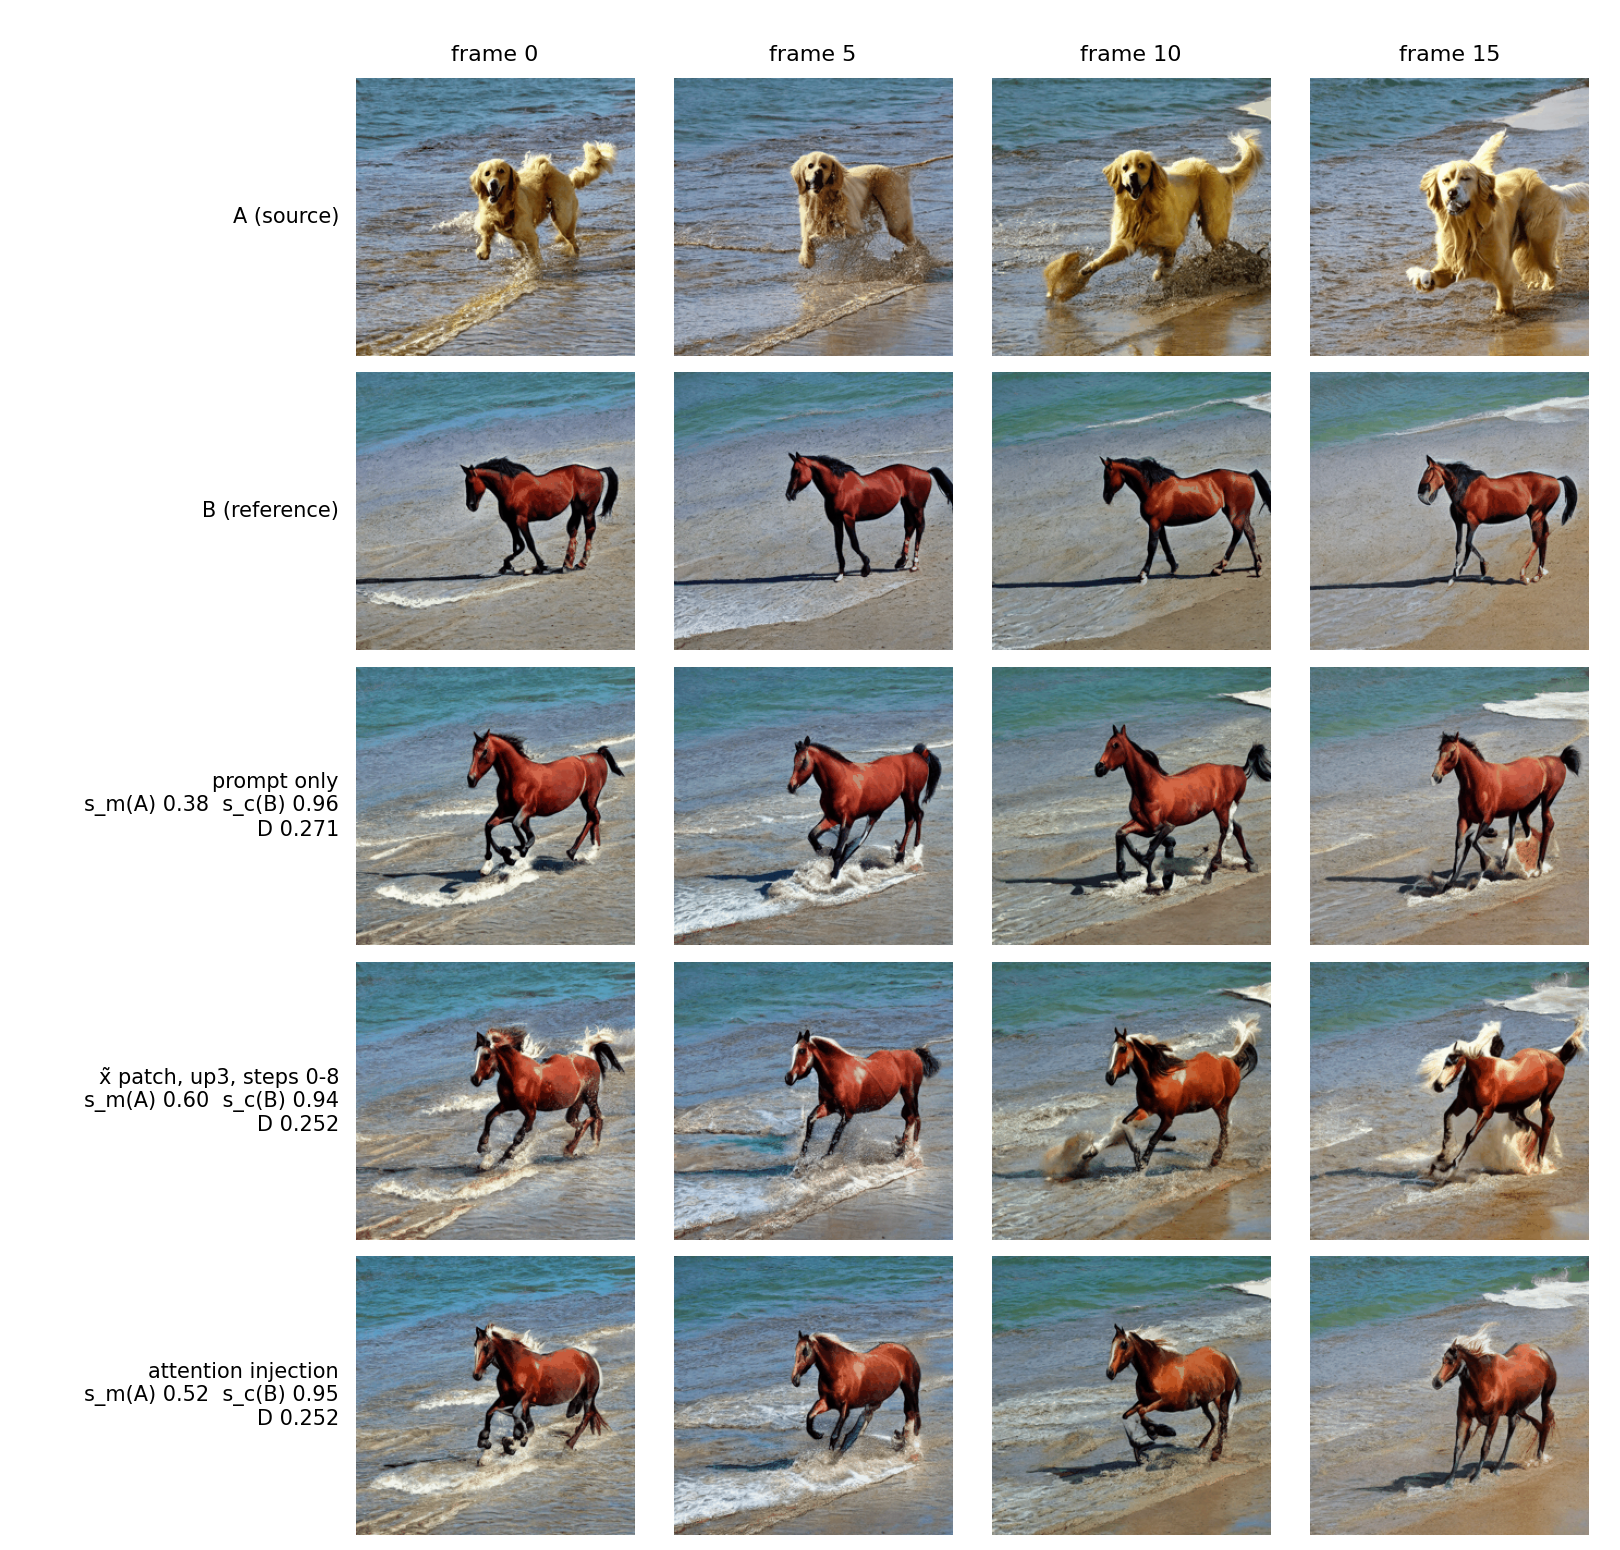
\includegraphics[width=0.86\textwidth]{figures/qual_motion_42.png}
	\caption{Motion direction on test pair 1 (``a golden retriever running'' $\to$ ``a horse walking'',
	beach, seed 42). Target prompt: ``a horse running''. The prompt-only horse runs, but in its own way;
	with the $\xd$ patch it picks up the dog's splash and stride, and its flow similarity to A rises from
	0.38 to 0.60. $D$ falls slightly on this pair because some of A's appearance comes along (the pale
	mane and spray).}
	\label{fig:qual_motion}
\end{figure}

\begin{figure}[!h]
	\centering
	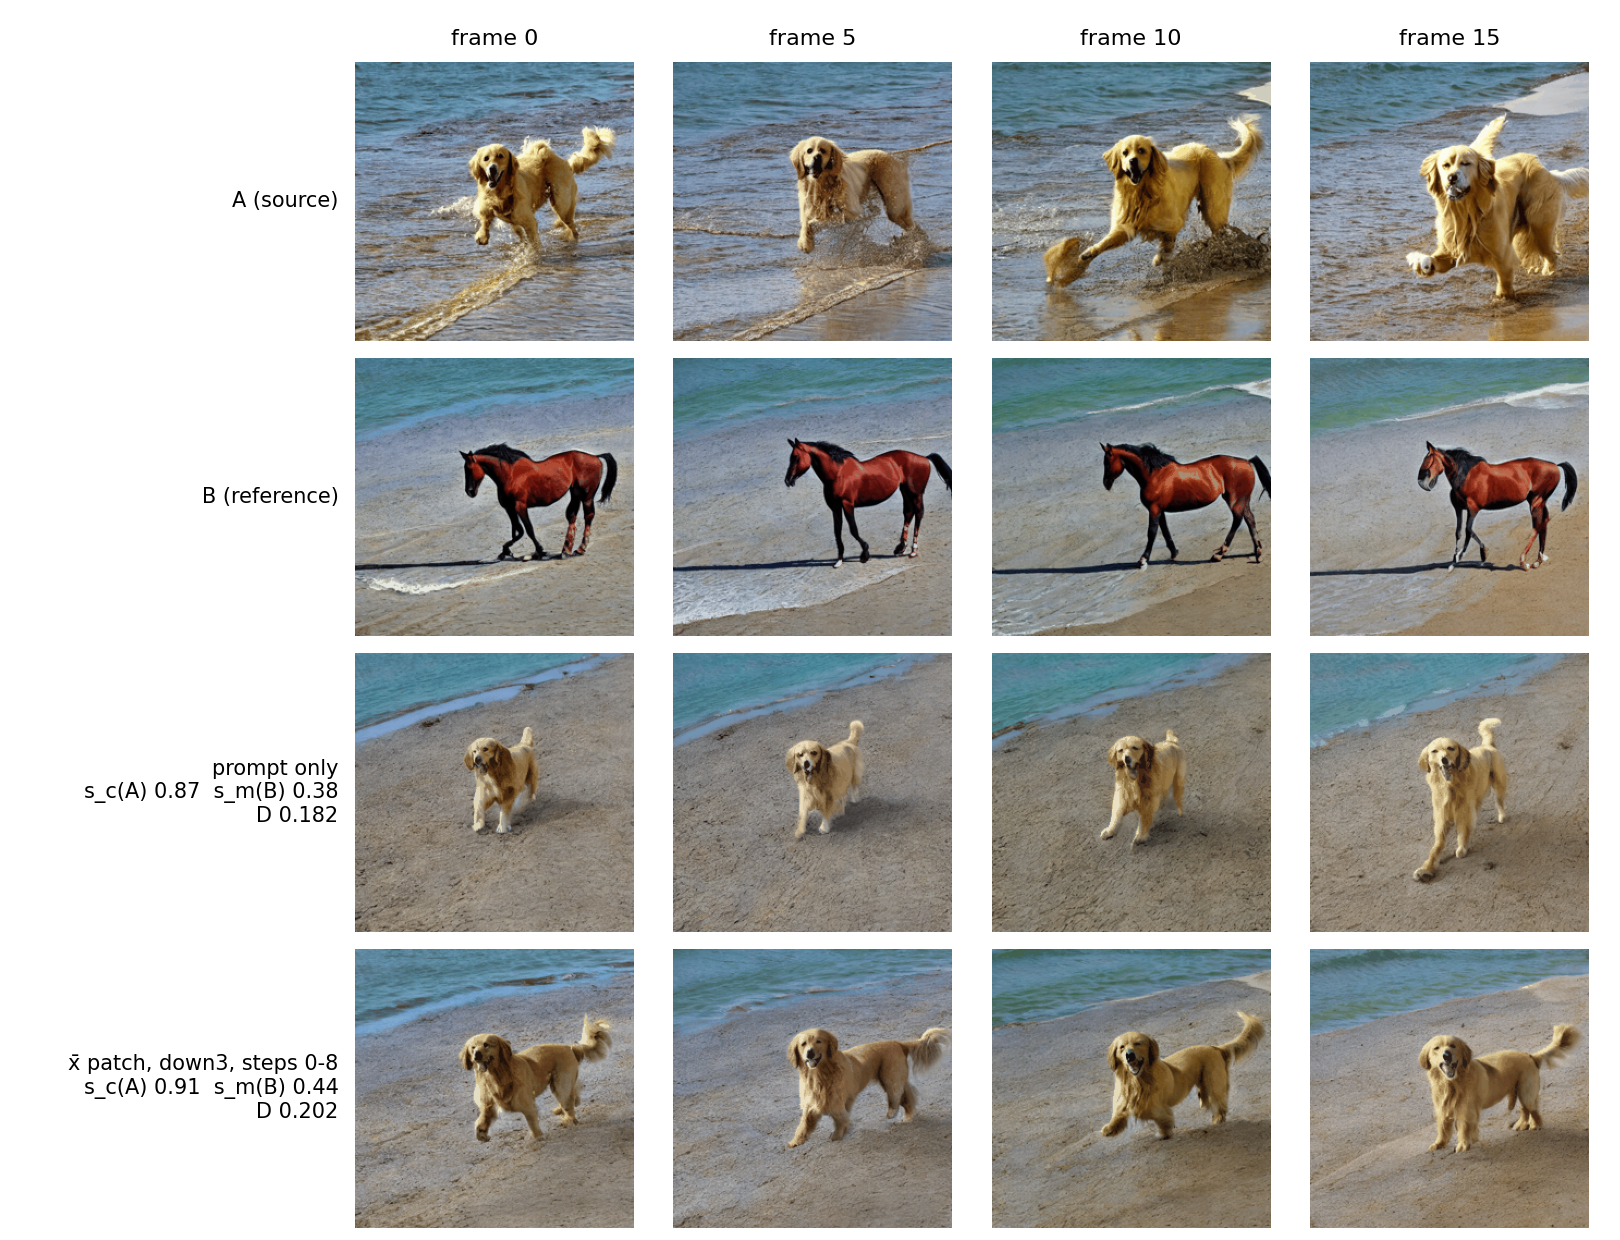
\includegraphics[width=0.86\textwidth]{figures/qual_content_42.png}
	\caption{Content direction on the same pair. Target prompt: ``a golden retriever walking''. The
	$\xs$ patch on \texttt{down\_blocks.3} keeps the source dog's build, coat and raised tail more closely
	than the prompt alone ($s_c$ to A 0.87 $\to$ 0.91) while it walks.}
	\label{fig:qual_content}
\end{figure}

Figures~\ref{fig:qual_motion} and \ref{fig:qual_content} show one pair in both directions. They also
show the limits of our metrics. CLIP similarity is a coarse measure of identity, and the flow cosine
rewards matching \emph{where} pixels move, which includes splashes and camera-like drift as well as the
animal's legs.

\subsection{Motion LoRAs}

\begin{table}[!h]
\centering
\small
\begin{tabular}{lccccc}
\toprule
 & & \multicolumn{2}{c}{Held-out loss at step 800} & \multicolumn{2}{c}{Test pairs, prompt + LoRA, median $\dD$} \\
Variant & Params & first recipe & cut-free, seeds 0/1/2 & first recipe & cut-free, per seed \\
\midrule
untrained & -- & 0.0996 & 0.0982 & -- & -- \\
\code{full}  & 9.67\,M & 0.0638 & 0.0627 / 0.0627 / 0.0627 & $-$0.021 & +0.004 / +0.008 / $-$0.013 \\
\code{probe} & 1.97\,M & 0.0652 & 0.0641 / 0.0641 / 0.0641 & +0.023 & +0.014 / +0.015 / +0.009 \\
\code{anti}  & 2.62\,M & 0.0646 & 0.0635 / 0.0636 / 0.0635 & $-$0.020 & $-$0.011 / $-$0.031 / $-$0.001 \\
\bottomrule
\end{tabular}
\caption{Motion LoRAs. The untrained loss differs between recipes because the cut-free validation
window is the centre of the longest shot. Cut-free $\dD$ is scored in one pool with the test run
(E10). Every $\dD$ CI in the table includes zero.}
\label{tab:lora}
\end{table}

\begin{figure}[!h]
	\centering
	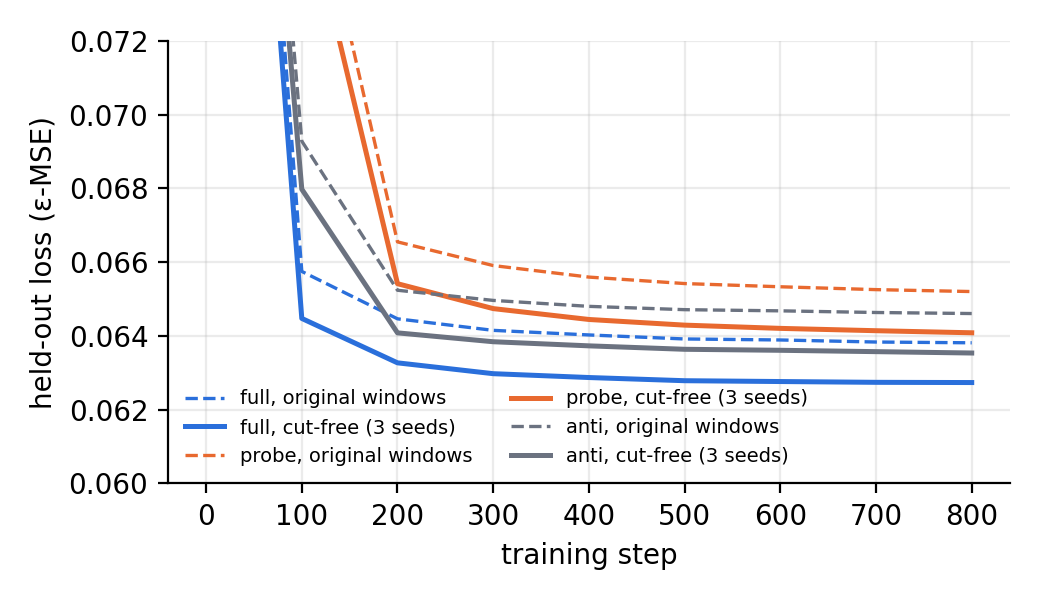
\includegraphics[width=0.62\textwidth]{figures/lora_val.png}
	\caption{Held-out loss during training. Most of the drop happens in the first 100 steps for every
	variant, which looks more like adapting to HMDB51's look (grain, low resolution) than to its motion.}
	\label{fig:lora_val}
\end{figure}

On held-out loss, placement matters less than size. In both recipes \code{full} is lowest and the
wrong-place control \code{anti} ends \emph{below} the map-guided \code{probe}, with 33\% more
parameters. The ordering is identical for all three cut-free seeds, and the spread between seeds is
below $10^{-4}$, so it is not noise. The validation loss is not specific to motion, though
(Figure~\ref{fig:lora_val}). The edit test is the better measure, and there the first-recipe
\code{probe} LoRA had the only positive median $\dD$ of the three. The cut-free retrain repeats
this: \code{probe} is positive in all three seeds (+0.009 to +0.015, 6--7 of 12 pairs), while
\code{full} and \code{anti} scatter around zero. So on the edit test the map-guided placement does
come out ahead, consistently but by a small margin, and no single CI excludes zero. The raw scores
qualify the gain. With \code{probe}, $s_m(\text{out},A)$ \emph{falls} from 0.23 to 0.14--0.17 while
$s_m(\text{out},B)$ falls further, from 0.17 to 0.06--0.08. The LoRA makes the clip move less like B
rather than more like A. That is what we should expect: it learned generic HMDB51 running,
walking, jumping and turning, not clip A's particular motion, so we compare the three LoRAs with one
another and not with the patches.

\textbf{What the full LoRA learns, block by block.} For the \code{full} LoRA we computed the relative
update $\|\Delta W\|_F / \|W\|_F$ per temporal block and ranked the nine blocks by it, by selectivity
$M(b)$, by verb-probe accuracy on $\xd$ and by usefulness for patching (dev $\dD$). The LoRA's largest
updates follow the probe ranking (Spearman +0.83, $p = 0.005$), peaking at \code{up_blocks.0} where
both the map and the probe peak; they do not follow patching usefulness ($-$0.27). The three
low-resolution blocks have larger relative updates in general, so part of this agreement may be
resolution rather than motion; we have not separated the two.

\subsection{Upload path} \label{sec:res_upload}

\begin{table}[!h]
\centering
\small
\begin{tabular}{lcccc}
\toprule
New clip starts from & prompt only & selected $\xd$ patch & attention, steps 0--8 & attention, all steps \\
\midrule
inverted noise & 0.118 & 0.519 (hybrid, artefacts) & 0.309 & \textbf{0.668} \\
blend of inverted and Gaussian & 0.322 & 0.025 (diverges) & 0.395 & \textbf{0.656} \\
Gaussian noise & 0.085 & 0.087 (diverges) & $-$0.053 & 0.366 \\
\bottomrule
\end{tabular}
\caption{Uploaded video (a baseball pitch) turned into ``a tiger jumping'': flow cosine of the new clip
to the upload. CLIP match to the target prompt is 0.33--0.36 for every clip that did not diverge.}
\label{tab:upload}
\end{table}

The component patch does not survive this setting (Table~\ref{tab:upload}). Logging norms inside the
patcher showed why. For a generated pair the frame-varying parts of source and target already agree
closely, since both start from the same noise, so the patch is a small nudge. For an uploaded video
they are unrelated: the difference at \code{up_blocks.3} is up to 12{,}400 against an output norm of
8--21 thousand at step 0, the target's norm grows every step, and the final latent has a standard
deviation of 26 instead of 0.7. The patch is a tool for pairs that share their initial noise, not a
layout-free motion transplant. The interface therefore defaults to attention injection over all steps
from the blended start. A second clip exposed another limit: a woman walking towards the camera became
a scene that grows towards the camera, while the robot in it stayed small and nearly still. Temporal
attention carries \emph{where} things move in the frame, not \emph{which object} moves.

\subsection{Interface}

All four tabs were checked through the running app with the same handlers as the buttons. A live
edit (4 clips) takes 4.5--7 minutes on the laptop GPU at 6.4\,GB peak; an upload edit about 4.5 minutes;
the results browser and the maps need no GPU. Invalid combinations (attention injection in the content
direction) are rejected with a message rather than an error.

\section{Plan for Novelty Assessment} \label{sec:Plan for Novelty Assessment}

The results leave four open questions, and the plan follows them.
\begin{enumerate}
\item \textbf{Is the split an artefact of AnimateDiff's training recipe?} Its spatial layers were frozen
  while the motion module was trained, so content \emph{had} to stay in the spatial path. We will run the
  same sweep (same vocabulary, same tests) on a model trained jointly on space and time, such as
  ModelScope T2V or VideoCrafter2. If H1--H3 come out the same, the map describes video diffusion; if not,
  it describes AnimateDiff.
\item \textbf{Combine what each method is good at.} Attention injection transfers \emph{where} things move,
  and the $\xd$ patch carries \emph{which} motion at the cost of some appearance. A combined arm, attention
  injection with a mask from the subject's cross-attention so that motion lands on the object, is the
  most direct fix for the failure in the upload path, and can be tested on the same 12 pairs.
\item \textbf{Statistical power.} Several arms have 9--10 of 12 positive pairs and CIs that miss zero by
  less than 0.03. We will add a second set of 24 pairs drawn by the same rule and report both sets, and
  run the symmetry control on all of them instead of one pair.
\item \textbf{Better measurements.} Replace optical-flow cosine with point tracks (CoTracker
  \citep{karaev2024cotracker}) and CLIP with DINO features for identity, and separate the resolution effect
  in the LoRA update ranking by normalising per resolution level.
\end{enumerate}

\section{Conclusion} \label{sec:conclusion}

We asked where a video diffusion U-Net keeps content and where it keeps motion, using AnimateDiff and a
controlled set of 750 one-word-swap pairs generated from shared noise. The answer is narrower than the
architecture suggests. Content dominates almost every layer, temporal ones included. Motion is selective
in only one place, the motion module just after the bottleneck, and only during the first two or three of
25 denoising steps. Removing the frame mean shifts every layer towards motion but reveals no hidden motion
layer, and two of our three pre-registered hypotheses were falsified. Turning the same static/dynamic
split into a patch gives edits that beat changing the prompt and beat whole-tensor patching in both
directions, but not by a margin that 12 test pairs can confirm. Temporal attention injection did
better, and over all 25 steps it is the one edit whose gain is clearly above zero. Where the map says
motion is represented is not where patching works best. A LoRA placed by the map was not better on
held-out loss than one placed where the map says motion is absent, but it was the only placement that
improved the edit in all three seeds, by a small margin. The
measurements are exact (null patches are bit-identical) and every decision was fixed before the data it
affected, so the negative results are results. All code, the LoRAs and an interface for trying the edits
are released with this report.

\begin{thebibliography}{99}
\setlength{\itemsep}{1pt}
\small

\bibitem{baherwani2025timesteps} Vatsal Baherwani, Yixuan Ren, and Abhinav Shrivastava. Characterizing motion encoding in video diffusion timesteps, arXiv preprint, 2025. \url{https://arxiv.org/abs/2512.22175}

\bibitem{blattmann2023align} Andreas Blattmann, Robin Rombach, Huan Ling, Tim Dockhorn, Seung Wook Kim, Sanja Fidler, and Karsten Kreis. Align your latents: High-resolution video synthesis with latent diffusion models, IEEE/CVF Conference on Computer Vision and Pattern Recognition (CVPR), 2023. \url{https://arxiv.org/abs/2304.08818}

\bibitem{farneback2003} Gunnar Farneb\"ack. Two-frame motion estimation based on polynomial expansion, Scandinavian Conference on Image Analysis (SCIA), 2003. \url{https://doi.org/10.1007/3-540-45103-X_50}

\bibitem{guo2024animatediff} Yuwei Guo, Ceyuan Yang, Anyi Rao, Zhengyang Liang, Yaohui Wang, Yu Qiao, Maneesh Agrawala, Dahua Lin, and Bo Dai. AnimateDiff: Animate your personalized text-to-image diffusion models without specific tuning, International Conference on Learning Representations (ICLR), 2024. \url{https://arxiv.org/abs/2307.04725}

\bibitem{hertz2023p2p} Amir Hertz, Ron Mokady, Jay Tenenbaum, Kfir Aberman, Yael Pritch, and Daniel Cohen-Or. Prompt-to-prompt image editing with cross attention control, International Conference on Learning Representations (ICLR), 2023. \url{https://arxiv.org/abs/2208.01626}

\bibitem{ho2022vdm} Jonathan Ho, Tim Salimans, Alexey Gritsenko, William Chan, Mohammad Norouzi, and David J. Fleet. Video diffusion models, Advances in Neural Information Processing Systems (NeurIPS), 2022. \url{https://arxiv.org/abs/2204.03458}

\bibitem{hu2022lora} Edward J. Hu, Yelong Shen, Phillip Wallis, Zeyuan Allen-Zhu, Yuanzhi Li, Shean Wang, Lu Wang, and Weizhu Chen. LoRA: Low-rank adaptation of large language models, International Conference on Learning Representations (ICLR), 2022. \url{https://arxiv.org/abs/2106.09685}

\bibitem{karaev2024cotracker} Nikita Karaev, Ignacio Rocco, Benjamin Graham, Natalia Neverova, Andrea Vedaldi, and Christian Rupprecht. CoTracker: It is better to track together, European Conference on Computer Vision (ECCV), 2024. \url{https://arxiv.org/abs/2307.07635}

\bibitem{kuehne2011hmdb} Hildegard Kuehne, Hueihan Jhuang, Est\'ibaliz Garrote, Tomaso Poggio, and Thomas Serre. HMDB: A large video database for human motion recognition, IEEE International Conference on Computer Vision (ICCV), 2011. \url{https://doi.org/10.1109/ICCV.2011.6126543}

\bibitem{ling2025motionclone} Pengyang Ling, Jiazi Bu, Pan Zhang, Xiaoyi Dong, Yuhang Zang, Tong Wu, Huaian Chen, Jiaqi Wang, and Yi Jin. MotionClone: Training-free motion cloning for controllable video generation, International Conference on Learning Representations (ICLR), 2025. \url{https://arxiv.org/abs/2406.05338}

\bibitem{meng2022rome} Kevin Meng, David Bau, Alex Andonian, and Yonatan Belinkov. Locating and editing factual associations in GPT, Advances in Neural Information Processing Systems (NeurIPS), 2022. \url{https://arxiv.org/abs/2202.05262}

\bibitem{radford2021clip} Alec Radford, Jong Wook Kim, Chris Hallacy, Aditya Ramesh, Gabriel Goh, Sandhini Agarwal, Girish Sastry, Amanda Askell, Pamela Mishkin, Jack Clark, Gretchen Krueger, and Ilya Sutskever. Learning transferable visual models from natural language supervision, International Conference on Machine Learning (ICML), 2021. \url{https://arxiv.org/abs/2103.00020}

\bibitem{rombach2022ldm} Robin Rombach, Andreas Blattmann, Dominik Lorenz, Patrick Esser, and Bj\"orn Ommer. High-resolution image synthesis with latent diffusion models, IEEE/CVF Conference on Computer Vision and Pattern Recognition (CVPR), 2022. \url{https://arxiv.org/abs/2112.10752}

\bibitem{song2021ddim} Jiaming Song, Chenlin Meng, and Stefano Ermon. Denoising diffusion implicit models, International Conference on Learning Representations (ICLR), 2021. \url{https://arxiv.org/abs/2010.02502}

\bibitem{tang2023daam} Raphael Tang, Linqing Liu, Akshat Pandey, Zhiying Jiang, Gefei Yang, Karun Kumar, Pontus Stenetorp, Jimmy Lin, and Ferhan Ture. What the DAAM: Interpreting Stable Diffusion using cross attention, Annual Meeting of the Association for Computational Linguistics (ACL), 2023. \url{https://arxiv.org/abs/2210.04885}

\bibitem{wang2023ioi} Kevin Wang, Alexandre Variengien, Arthur Conmy, Buck Shlegeris, and Jacob Steinhardt. Interpretability in the wild: A circuit for indirect object identification in GPT-2 small, International Conference on Learning Representations (ICLR), 2023. \url{https://arxiv.org/abs/2211.00593}

\bibitem{wu2023tav} Jay Zhangjie Wu, Yixiao Ge, Xintao Wang, Stan Weixian Lei, Yuchao Gu, Yufei Shi, Wynne Hsu, Ying Shan, Xiaohu Qie, and Mike Zheng Shou. Tune-A-Video: One-shot tuning of image diffusion models for text-to-video generation, IEEE/CVF International Conference on Computer Vision (ICCV), 2023. \url{https://arxiv.org/abs/2212.11565}

\bibitem{xiao2024moft} Zeqi Xiao, Yifan Zhou, Shuai Yang, and Xingang Pan. Video diffusion models are training-free motion interpreter and controller, Advances in Neural Information Processing Systems (NeurIPS), 2024. \url{https://arxiv.org/abs/2405.14864}

\bibitem{yatim2024dmt} Danah Yatim, Rafail Fridman, Omer Bar-Tal, Yoni Kasten, and Tali Dekel. Space-time diffusion features for zero-shot text-driven motion transfer, IEEE/CVF Conference on Computer Vision and Pattern Recognition (CVPR), 2024. \url{https://arxiv.org/abs/2311.17009}

\bibitem{zhang2024patching} Fred Zhang and Neel Nanda. Towards best practices of activation patching in language models: Metrics and methods, International Conference on Learning Representations (ICLR), 2024. \url{https://arxiv.org/abs/2309.16042}

\bibitem{zhao2024motiondirector} Rui Zhao, Yuchao Gu, Jay Zhangjie Wu, David Junhao Zhang, Jiawei Liu, Weijia Wu, Jussi Keppo, and Mike Zheng Shou. MotionDirector: Motion customization of text-to-video diffusion models, European Conference on Computer Vision (ECCV), 2024. \url{https://arxiv.org/abs/2310.08465}

\bibitem{hf_animatediff} Yuwei Guo and others. \url{https://huggingface.co/guoyww/animatediff-motion-adapter-v1-5-2}, Accessed on: 20th October, 2026.

\bibitem{hf_diffusers} Hugging Face. \url{https://huggingface.co/docs/diffusers}, Accessed on: 20th October, 2026.

\bibitem{hf_hmdb} DIVM. \url{https://huggingface.co/datasets/divm/hmdb51}, Accessed on: 20th October, 2026.

\end{thebibliography}

\end{document}
